\documentclass[12pt,a4paper]{article}
%\documentclass[8pt]{beamer}
%\usetheme{default}
%\usepackage[font=small,format=plain,labelfont=bf,up,textfont=it,up]{caption}
%\usepackage{setspace}
\usepackage{graphicx}
\usepackage{epstopdf}
\usepackage{natbib}
\bibpunct{(}{)}{;}{a}{}{,}
\usepackage[brazil]{babel}
\usepackage[utf8]{inputenc}
\usepackage {enumerate}
\usepackage{latexsym}
\usepackage{amsmath}
%\usepackage[T1]{fontenc}
%\usepackage{fetamont}
%\usepackage[num]{abntcite}
\usepackage{ mathrsfs }
\usepackage{subfigure}
\usepackage{helvet}
\renewcommand{\familydefault}{\sfdefault}

\newcommand{\farcm}{\mbox{\ensuremath{.\mkern-4mu^\prime}}}%
\newcommand{\farcs}{\mbox{\ensuremath{.\!\!^{\prime\prime}}}}
\newcommand{\ii }{\'{\i}}
\newcommand{\cc }{\c c}
\newcommand{\cca}{\c ca }
\newcommand{\ao}{\~ao }
\newcommand{\cao}{\c c\~ao }
\newcommand{\oes}{\~oes }
\newcommand{\coes}{\c c\~oes }
\newcommand{\eq}{\begin{equation}}
\newcommand{\feq}{\end{equation}}
\newcommand{\dm}{\begin{displaymath}}
\newcommand{\fdm}{\end{displaymath}}
\newcommand{\eqn}{\begin{eqnarray}}
\newcommand{\feqn}{\end{eqnarray}}
\newcommand{\grau}{^{\circ}}
\newcommand{\ba}{\arrowvert_{t_1}^{t_2}}
\newcommand{\bc}{\arrowvert_{0^{\circ} {\rm C}}^{t_2}}
\newcommand{\bb}{\arrowvert_{0^{\circ} {\rm C}}^{t_1}}
\newcommand{\Ms}{$\mathrm{M}_{\odot}$}
%\renewcommand{\labelitemiv}{$-$}
\usepackage{amssymb}
\newcommand{\reg}[1]{#1$^{\tiny{\circledR}}$}
\usepackage[hmargin=2cm,vmargin=2.5cm,bmargin=2cm]{geometry}
\renewcommand{\baselinestretch}{1.2}
%\topmargin -1.5cm
%\leftmargin -2cm
%\rightmargin -2cm
%\oddsidemargin -0.7cm
%\textwidth 16cm
%\textheight 24cm
%\hoffset -1cm 

\usepackage{epic}
\usepackage{arydshln}
\providecommand{\sin}{} \renewcommand{\sin}{\hspace{2pt}\mathrm{sen}}
\numberwithin{equation}{section}

\begin{document}

% CAPA

\thispagestyle{empty}

  \begin{figure}[!htb]
    \centering
    \includegraphics[scale=0.2]{ufmg.jpg}
    \label{figRotulo}
  \end{figure}

\vspace{3 mm}
\begin{center}
{ESCOLA DE ENGENHARIA}\\
{PROGRAMA DE PÓS-GRADUAÇÃO EM ENGENHARIA ELÉTRICA}\\
\end{center}

\vspace{15mm}
\begin{center}
Luiz Alberto Queiroz Cordovil Júnior \\
Rodrigo Farias Araújo
\end{center}

\vspace{50 mm}
\begin{center}
\textbf{Exercício Computacional 2}\\
\end{center}

\vspace{30 mm}

\vspace{60mm}
\begin{center}
Belo Horizonte - MG\\
Setembro - 2017
\end{center}
\thispagestyle{empty}
\newpage

%CONTRA-CAPA

\thispagestyle{empty}

\vspace{3 mm}
\begin{center}
Luiz Alberto Queiroz Cordovil Júnior \\
Rodrigo Farias Araújo
\end{center}


\vspace{45 mm}
\begin{center}
\textbf{Effect of Rule Weights in Fuzzy Rule-Based \\
Classification Systems}\\
\end{center}

\vspace{25 mm}

\vspace{35mm}
\hspace{9cm}\begin{minipage}[r]{0.45\linewidth}
Trabalho apresentado como parte das exigências para obtenção de nota parcial junto à disciplina Sistemas Nebulosos do PPGEE-UFMG, no S2/2017.\\ 
\\
Prof. Dr. André Paim Lemos
\end{minipage}

\vspace{60mm}
\begin{center}
Belo Horizonte - MG\\
Setembro - 2017

\end{center}

\thispagestyle{empty}
\newpage
\tableofcontents
\newpage

\abstract
Este trabalho apresenta a reprodução da metodologia e dos procedimentos experimentais realizados no artigo de Hisao Ishibuchi e Tomoharu Nakashima (2001), denominado \textit{Effect of Rule Weights in Fuzzy Rule-Baes Classification Systems}, em que são avaliados os efeitos de ponderação de regras em sistemas de classificação fuzzy. A metodologia considera que os valores linguísticos antecedentes de cada classe tem uma única classe consequente, a partir da observação de grau de compatibilidade e de certeza, quando da classificação de padrões. Os autores reivindicam que sistemas de classificação fuzzy com alta performance podem se projetados sem modificar as funções de pertinência de valores linguísticos antecedentes, quando do uso de ponderação de regras com graus de certeza.
\newpage

\section{Introdução}


De maneira geral os problemas de classificação são aproximações baseadas em dados  no sentido de mapear classes de um conjunto de variáveis. Em sistemas baseados em regras fuzzy, a identificação de padrões e consequente classificação a partir de um número finito (\textit{n}) de atributos é definido como:

\begin{equation} \label{eq1}
Regra~R_{j}:~Se~x_{1}~ \text{é }A_{j1}~e... e~x_{n}~\text{é }A_{jn}~\text{então } Classe~C_{j},~j=1,2,...,N
\end{equation}
em que:
\begin{itemize}
\item $x={x_{1},...,x_{n}}$: $n-$dimensional vetor de padrões;
\item $A_{ij}$: valor linguístico antecedente como "grande" e "pequeno" $~(i=1,2,...,n)$;
\item $C_{j}$: classe consequente;
\item $N$: número de regras fuzzy SE-ENTÃO.
\end{itemize}

Na abordagem do artigo a ponderação das regras SE-ENTÃO com certos graus de certeza é dada por:

\begin{equation} \label{eq2}
Regra~R_{j}:~Se~x_{i}~\text{é } A_{j1}~e...e~x_{n} \text{é } A_{jn}~\text{então }Classe~C_{j}~com~CF_{j}, j=1,2,...,N
\end{equation}
em que:
\begin{itemize} 
\item $CF_{j}$ é o grau de certeza de cada regra fuzzy SE-ENTÃO $R_{j}$, e, usualmente é um número real no intervalo [0,1].
\end{itemize}

Para esta aplicação foi utilizada a base de dados Iris (1936), do biólogo e estatístico britânico Ronald Fisher, para três espécies da flor \textit{Iris} (\textit{50 setosa, 50 virginica, 50 versicolor}). Considera-se o conjunto de dados separáveis pela discriminação das seguintes características:

\begin{itemize}
\item comprimento e largura da sépala;
\item comprimento e largura da pétala.
\end{itemize}

\section{Metodologia}

O método implementado consiste de uma abordagem de seleção de apenas uma classe, ou classe vencedora, durante a fase de classificação, além de, quando na observação da área de decisão haver fronteiras de classificação tendo em vista as regras fuzzy. Ao ponderar-se estas pelo grau de certeza $C_{j}$:

\begin{equation} \label{eq3}
\sum_{p\in Class~C_{j}} \mu_{j}(x_p)=\max(\sum_{p\in Class~k}\mu(x_{p}):k=1,2,...,c)
\end{equation}
em que:

$x_{p}$: número de padrões;

$c$: número de classes.

Como poder visto na equação (\ref{eq3}) a classe consequente $C_{j}$ é especificada como a classe dominante no espaço fuzzy correspondente ao antecedente de cada regra fuzzy SE-ENTÃO. Aplicando-se a definição demonstrada na equação (\ref{eq2}), um novo padrão $x{p}=(x_{p1},...,x_{pn}))$, pode ser definido como:

\begin{equation} \label{eq4}
\mu_{j}^{ *}(x_{p}).CF_{j}=\max\lbrace\mu_{j}(x_{p}).CF_{j}:~j=1,2,...,N\rbrace
\end{equation}

A classe consequente pode ser determinada partir de padrões de treinamento, como também se esta é a dominante. Na abordagem computacional, por meio da técnica de validação cruzada, em que separou-se cada conjunto de espécies em subconjuntos de treinamento e teste representados por  70\% e 30\%, respectivamente de cada classe de padrões. 

Como todo regra tem sua própria área de decisão, cujo tamanho é determinado pelo grau de certeza e pelo antecedente linguístico das funções de pertinência, a abordagem realiza mudança na dimensão da área de decisão por ponderação sem alterar as funções de pertinência. Neste sentido o grau de certeza é dado por:

\begin{equation} \label{eq5}
CF_{j}=\frac{\beta_{Classe~C_{j}}(R_{j})-\overline{\beta}}{\sum_{k=1}^{c}\beta_{Classe~k}(R_{j})}
\end{equation}
em que $C_{j}$ é a classe consequente e:

\begin{equation} \label{eq6}
\overline{\beta}=\frac{\sum_{k\neq C_{j}}\beta_{Classe~k}(R_{j})}{(c-1)}
\end{equation}

As formulações indicadas nas equações (\ref{eq5}) e (\ref{eq6})  estendem a determinação do grau de certeza para um problema de classificação com $c$ classes.

\subsection{Procedimentos Computacionais}

\begin{figure}[ht]
\centering
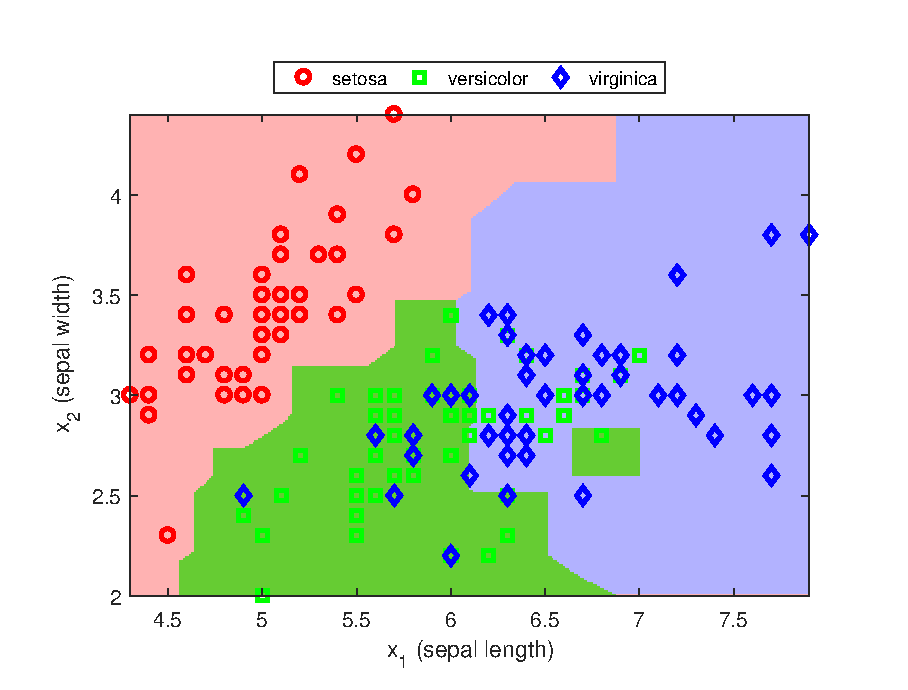
\includegraphics[width=0.7\textwidth]{product.eps}
\caption{Região de decisão usando a t-norma produto.}
\label{fig:produst}
\end{figure}

lhhkjhkjhkhkj

\newpage
\section{Conclusões}

Neste trabalho foram apresentados e implementados cinco métodos clássicos de solução
do problema de fluxo de carga em redes de sistemas elétricos.
Os métodos foram testados em dois estudos de caso de sistemas de duas barras e num sistema
de 4 barras (B4).
A aplicação dos métodos aos dois estudos de caso apresentaram resultados satisfatórios
e o comportamento de convergência dos métodos foi como esperado. 
No entanto, a aplicação dos métodos ao sistema B4, que é a proposta do trabalho, não 
resultou em convergência. A não-convergência pode ser devido ao fato de que não foi
realizado o controle das tensões nas barras. 

\newpage

\section*{Referências}
\addcontentsline{toc}{section}{\protect\numberline{}Referências}%

[1] ISHIBUCHI, Hisao; NAKASHIMA, Tomoharu. Effect of rule weights in fuzzy rule-based classification systems. IEEE Transactions on Fuzzy Systems, v. 9, n. 4, p. 506-515, 2001.

\end{document}
